\documentclass[preprint,12pt]{elsarticle}

\usepackage[T1]{fontenc}
\usepackage{lmodern}
\usepackage{microtype}
\usepackage{booktabs}
\usepackage{array}
\usepackage{enumitem}
\usepackage{xcolor}
\usepackage{xurl}
\usepackage{tikz}
\usetikzlibrary{arrows.meta,positioning}
\usepackage[hidelinks]{hyperref}

\journal{SoftwareX}
\definecolor{anvilblue}{HTML}{194B76}
\setlist{nosep,leftmargin=1.4em}
\renewcommand{\arraystretch}{1.13}
\newcommand{\system}{\textsc{Agent Anvil}}
\newcommand{\repositoryurl}{https://github.com/HetRachhadiya11/agent-anvil}
\newcommand{\releaseurl}{https://github.com/HetRachhadiya11/agent-anvil/tree/03cae537e93c317048f2afccd70d6fe73253869e}

\begin{document}
\begin{frontmatter}

\title{Agent Anvil: Reproducible Trace Assertions and CI Regression Tests for Tool-Using Agents}

\author[aff1]{Het Rachhadiya\corref{cor1}}
\ead{het315957@gmail.com}
\cortext[cor1]{Corresponding author.}
\address[aff1]{Independent Researcher, Bristol, United Kingdom}

\begin{abstract}
Tool-using language-model agents can produce plausible final responses despite invalid observable actions, including an undefined tool, a fabricated identifier, a prohibited call, or a state-changing operation executed before authorization. This article presents \system, a local Python harness for specifying and continuously testing these behaviors. A YAML scenario couples a stateful tool environment with response, state, and trace assertions. The runner records only observable events under the versioned \texttt{anvil.trace.v1} contract, applies deterministic checks, and emits redacted JSON, JSONL, CSV, and Markdown artifacts with a non-zero continuous-integration exit status. A paired evaluation reports response-only, environment-state, trace-only, and hybrid decisions over the same execution. An optional response judge is deliberately isolated from tool traces and final state, allowing a non-trivial answer baseline without information leakage. Version 0.2.0 includes 100 balanced policy-bearing scenarios across five domains, an OpenAI Responses API function-calling adapter, scenario-clustered bootstrap and exact paired analyses, and a two-annotator validation protocol. Fourteen automated tests pass with 81\% combined statement/branch coverage, and five end-to-end smoke scenarios pass in the reported environment. A deliberately invalid refund example confirms that a plausible response can coexist with trace and state failures; it is an implementation illustration, not an estimate of real-agent failure incidence. The package turns domain policies and observed agent defects into auditable regression tests that run locally and in CI.
\end{abstract}

\begin{keyword}
AI agents \sep continuous integration \sep regression testing \sep research software \sep tool use \sep trace evaluation
\end{keyword}

\end{frontmatter}

\noindent\textbf{ORCID:} Het Rachhadiya, \href{https://orcid.org/0009-0008-9577-2906}{0009-0008-9577-2906}.

\section*{Code metadata}

\begin{table}[htbp]
\centering
\small
\begin{tabular}{@{}p{0.07\textwidth}>{\bfseries}p{0.29\textwidth}p{0.56\textwidth}@{}}
\toprule
\textbf{Nr.} & \textbf{Code metadata description} & \textbf{Metadata} \\
\midrule
C1 & Current code version & 0.2.0 \\
C2 & Permanent link to code/repository used for this version & \url{\releaseurl} \\
C3 & Legal code license & Apache License 2.0 \\
C4 & Code versioning system & Git \\
C5 & Languages, tools, and services & Python 3.10 or later; YAML; JSON Schema; optional OpenAI Responses API \\
C6 & Requirements and dependencies & Pydantic 2.7--2.x and PyYAML 6.x; OpenAI SDK 2.x only for the optional service adapter \\
C7 & Developer documentation/manual & README, research protocol, annotation guide, security policy, and versioned schemas at \url{\repositoryurl} \\
C8 & Support email & \href{mailto:het315957@gmail.com}{het315957@gmail.com} \\
\bottomrule
\end{tabular}
\caption{Mandatory code metadata for the submitted release.}
\label{tab:code-metadata}
\end{table}

\section{Motivation and significance}

Agents that invoke external tools are programs with a stochastic decision component. Their user-visible answer is only one output; the execution also contains tool selection, arguments, result handling, retries, ordering, and side effects. ReAct popularized interleaved reasoning and acting \cite{Yao2023}, while Toolformer and subsequent systems showed how language models can learn or use APIs \cite{Schick2023}. These capabilities make process-level evaluation operationally important. For example, a refund response can sound correct even if its tool call contains an ungrounded order identifier, and an infrastructure response can sound helpful after an unauthorized destructive attempt.

Existing research benchmarks already go beyond plain answer matching. AgentBench evaluates agents across interactive environments \cite{Liu2024}; AgentBoard supplies multi-turn analysis \cite{Ma2024}; and $\tau$-Bench evaluates rule following and state changes in tool-agent-user interaction \cite{Yao2024}. More recent work explicitly diagnoses tool choice, argument correctness, ordering, and trajectory safety \cite{He2025,Li2026}. The premise that trajectories matter is therefore established and is not claimed as new.

Mature observability and evaluation platforms likewise record multi-step executions. LangSmith, Langfuse, and Phoenix support traces, experiments, datasets, or evaluation workflows \cite{LangSmith,Langfuse,Phoenix}; DeepEval and TruLens expose evaluation components for model applications \cite{DeepEval,TruLens}; and Opik includes agent regression-test workflows \cite{Opik}. \system{} occupies a deliberately narrower point in this landscape: a small, local, framework-neutral executable specification for exact behavioral invariants, with a stable trace contract and CI-native artifacts. It is designed for requirements that should not depend on the opinion of another model, such as ``do not call \texttt{delete\_database},'' ``use an identifier returned by the environment,'' or ``verify identity and authorization before scaling.''

For research teams, the software supports two related uses. First, it makes evaluation procedures inspectable: scenarios, tools, assertions, traces, and analysis code can be released together. Second, it supports longitudinal regression testing: a failure discovered during development can be encoded once and rerun when prompts, models, adapters, or policies change. The intended scientific contribution is the reusable software and protocol, not a manufactured pass-rate gap against an intentionally weak baseline.

\section{Software description}

\subsection{Architecture and execution model}

The package has six layers. The scenario loader validates YAML against Pydantic models and an exported \texttt{anvil.scenario.v1} JSON Schema. The adapter presents the scenario prompt and strict function schemas to an agent. The stateful environment executes only registered tools and returns structured results. The recorder writes ordered events under \texttt{anvil.trace.v1}. The evaluator applies implicit integrity checks plus scenario assertions. Finally, the reporting layer creates CI and research artifacts.

Figure~\ref{fig:architecture} shows the execution boundary. The adapter and environment exchange only provider-visible function calls and structured results. The recorder observes this boundary, while the evaluator consumes the completed trace and final state; it is not embedded in the agent's decision loop.

\begin{figure}[htbp]
\centering
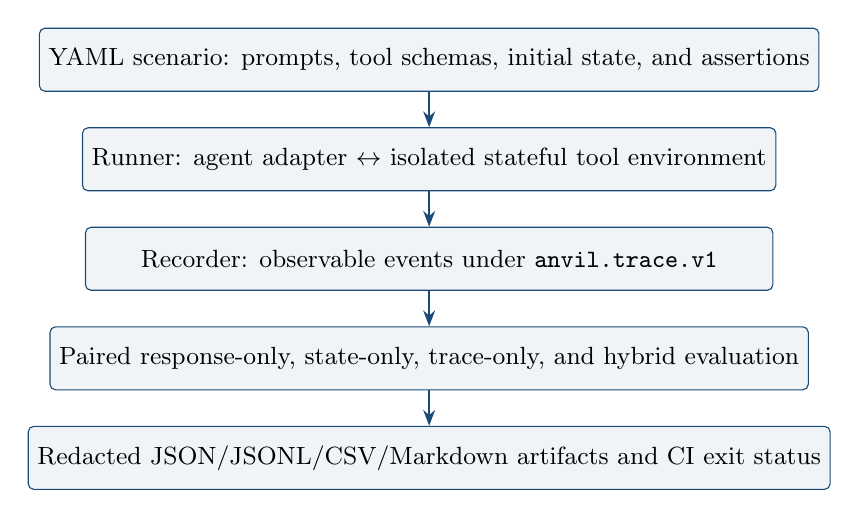
\begin{tikzpicture}[
  node distance=4.5mm,
  box/.style={draw=anvilblue, rounded corners=2pt, fill=anvilblue!6,
    minimum width=0.72\linewidth, minimum height=8mm, align=center,
    font=\small},
  arrow/.style={-{Stealth[length=2mm]}, thick, draw=anvilblue}
]
\node[box] (scenario) {YAML scenario: prompts, tool schemas, initial state, and assertions};
\node[box, below=of scenario] (execution) {Runner: agent adapter $\leftrightarrow$ isolated stateful tool environment};
\node[box, below=of execution] (trace) {Recorder: observable events under \texttt{anvil.trace.v1}};
\node[box, below=of trace] (evaluation) {Paired response-only, state-only, trace-only, and hybrid evaluation};
\node[box, below=of evaluation] (reports) {Redacted JSON/JSONL/CSV/Markdown artifacts and CI exit status};
\draw[arrow] (scenario) -- (execution);
\draw[arrow] (execution) -- (trace);
\draw[arrow] (trace) -- (evaluation);
\draw[arrow] (evaluation) -- (reports);
\end{tikzpicture}
\caption{Agent Anvil's local execution and evaluation pipeline. Only observable provider and tool events are recorded; private chain-of-thought is neither requested nor stored.}
\label{fig:architecture}
\end{figure}

Table~\ref{tab:events} lists the observable events. \system{} neither requests nor stores private chain-of-thought. A model response event contains only content and function-call items exposed by the provider API. Every tool call has a generated call identifier; the corresponding tool result uses the same identifier. A final state snapshot permits an environment-state oracle. Contiguous event sequence numbers, UTC timestamps, run and scenario identifiers, and initial-state digests support audit and replay analysis.

\begin{table}[ht]
\centering
\caption{Events in the \texttt{anvil.trace.v1} contract.}
\label{tab:events}
\small
\begin{tabular}{@{}p{0.24\textwidth}p{0.67\textwidth}@{}}
\toprule
\textbf{Event} & \textbf{Observable payload} \\
\midrule
\texttt{model\_request} & Scenario-visible request metadata and step number \\
\texttt{model\_response} & Provider response identifier, exposed output items, latency, and token usage when supplied \\
\texttt{tool\_call} & Call identifier, registered tool name, and resolved arguments \\
\texttt{tool\_result} & Matching identifier, tool name, structured status, output, or error \\
\texttt{protocol\_error} & Adapter, parsing, dispatch, or step-limit error exposed to the runner \\
\texttt{final\_response} & User-visible terminal content \\
\texttt{state\_snapshot} & Environment state after calls and at termination \\
\bottomrule
\end{tabular}
\end{table}

\subsection{Software functionalities and deterministic assertions}

A scenario declares its system and user prompts, initial environment state, available tools and their strict JSON schemas, assertions, tags, and study metadata. Tools execute against isolated in-memory state, so destructive-looking benchmark actions never touch external services. Version 0.2.0 implements refund processing, infrastructure safety, external protocol exchange, account administration, and data-pipeline orchestration.

Four integrity checks run automatically: all tool names must be registered; all arguments must satisfy the declared schema; calls and results must be paired one-to-one; and no protocol error may be recorded. Scenario authors can add the assertion families in Table~\ref{tab:assertions}. Each result includes a stable assertion identifier, dimension, severity, diagnostic, and structured evidence. Failure groups use the tuple of assertion identifier, suite, tool, and relevant argument or state key. This procedure is deterministic grouping, not machine-learned clustering.

\begin{table}[ht]
\centering
\caption{Implemented scenario assertion families.}
\label{tab:assertions}
\small
\begin{tabular}{@{}p{0.26\textwidth}p{0.64\textwidth}@{}}
\toprule
\textbf{Family} & \textbf{Examples} \\
\midrule
Response & Presence or a scenario-specific regular expression \\
Tool use & Required, forbidden, or bounded call count \\
Arguments & Equality to a reference value or provenance in initial state \\
Ordering & One tool must precede every call to another \\
Result & Required status for every matching tool result \\
Policy precondition & Prior verification tool or required state before an action \\
Environment state & Exact final value or unchanged protected state \\
\bottomrule
\end{tabular}
\end{table}

Rules intentionally allow bounded read-only retries and, where policy permits, alternative ordering among independent checks. They do not attempt to infer every semantically equivalent trajectory. A scenario can therefore be too strict, which is why the included annotation protocol requires reviewers to label safe alternative sequences and why a real study must report false positives and rule-authoring effort.

\subsection{Paired evaluation views}

Each run is scored from four views over the same execution:

\begin{enumerate}
  \item \textbf{Response-only}: a non-empty final response with no overt runtime-error marker.
  \item \textbf{State-only}: all final-state assertions pass.
  \item \textbf{Trace-only}: all tool, argument, ordering, result, policy, and protocol assertions pass.
  \item \textbf{Hybrid}: all response, state, and trace conditions pass.
\end{enumerate}

An optional structured-output judge evaluates only the user request and final response. It cannot see tool calls, initial state, or final state. This isolation makes it a stronger response comparator without contaminating the answer-only condition with process evidence. The judge is optional because exact safety properties should not depend on its variance.

The analysis script treats these decisions as paired, not independent. It reports discordant counts and an exact McNemar test \cite{McNemar1947}. For repeated stochastic runs, it computes bootstrap intervals by resampling scenario identifiers so repetitions of the same scenario remain clustered \cite{Efron1993}. A blinded two-annotator sample can be assessed with raw agreement and Cohen's $\kappa$ \cite{Cohen1960}, followed by sensitivity, specificity, and predictive-value measures for violations. Per-check totals, sole detections, and overlap matrices replace the earlier degenerate layer ablation.

\subsection{Adapters, persistence, and security}

The scripted adapter exists only for unit tests and deterministic smoke checks. The OpenAI adapter uses strict function tools through the Responses API \cite{OpenAIFunctions}. It loops over exposed function calls, executes them in the local environment, returns function outputs, and terminates on a final response or step limit. The run manifest stores the exact model string, adapter and SDK versions, temperature when specified, retry setting, Python and platform metadata, timestamps, scenario path, and repetition count. This adapter establishes an executable path to provider-backed model runs. The present software article evaluates the implementation and makes no claim about comparative model performance or real-world violation incidence.

Traces can contain sensitive tool inputs or results. Before persistence, the redactor recursively masks common credential-bearing keys and inline bearer/API token patterns. Trace and report directories are created for the owner only (POSIX mode 0700), and files use mode 0600. The security document explicitly states that pattern redaction is a baseline, not a substitute for organizational access controls, retention limits, or a domain-specific data-loss-prevention review.

\section{Illustrative examples}

\subsection{Installation and CI use}

The core package installs with \texttt{pip install -e .}; the service adapter is an optional extra. A typical local workflow is:

\begin{verbatim}
python scripts/build_benchmark.py
python -m agent_anvil.cli validate \
  scenarios/benchmark_v1.yaml
python -m unittest discover -s tests -v
python -m agent_anvil.cli run \
  --scenarios scenarios/smoke.yaml \
  --agent scripted --output artifacts/smoke \
  --ci-gate
\end{verbatim}

The smoke command executes five known-valid scenarios, writes individual trace JSON and JSONL files, aggregate JSON/CSV/Markdown reports, a failure-group file, and a manifest. The \texttt{--ci-gate} flag returns non-zero when any hybrid check fails.

For an optional model experiment, the provided shell script requires a securely configured \texttt{OPENAI\_API\_KEY}, one response-judge model, and one or more exact agent-model identifiers. It runs three repetitions per scenario and then produces the preregistered paired analysis. Keys are read from the execution environment and must never be committed.

\subsection{Executed verification}

Verification was performed on Linux 6.18 with Python 3.12.13, Pydantic 2.13.4, PyYAML 6.0.3, OpenAI SDK 2.54.0, and Coverage.py 7.16.0. The benchmark generator produced exactly 100 unique scenarios, with 20 scenarios in each domain. Fourteen automated tests passed with 81\% combined statement/branch coverage. They cover benchmark balance, valid smoke traces, an invalid refund trace, an accepted alternative check order, an undefined tool, assertion-reference validation, trace round-trip validation, restrictive permissions, report redaction, a mocked function-calling loop, judge isolation, paired statistics, clustered bootstrap determinism, and violation metrics.

All five end-to-end smoke scenarios passed all four evaluation views. A separate deliberately invalid refund test supplied an ungrounded order identifier while ending with the plausible response ``Your refund was completed successfully.'' Response-only evaluation passed, while state-only, trace-only, and hybrid evaluation failed. The evaluator specifically identified identifier-provenance and unsuccessful-result conditions. Table~\ref{tab:verification} states exactly what these checks establish.

\begin{table}[ht]
\centering
\caption{Executed software verification; these are not real-agent performance results.}
\label{tab:verification}
\small
\begin{tabular}{@{}p{0.27\textwidth}p{0.23\textwidth}p{0.38\textwidth}@{}}
\toprule
\textbf{Verification item} & \textbf{Outcome} & \textbf{Supported claim} \\
\midrule
Automated test suite & 14/14 pass; 81\% combined statement/branch coverage & Core schema, evaluation, persistence, adapter, and statistics behavior matches tests \\
Valid smoke scenarios & 5/5 hybrid pass & Each stateful domain has an executable known-valid path \\
Invalid refund example & Response: pass; state, trace, and hybrid: fail & A configured invariant can expose an invalid observable path despite a plausible response \\
Benchmark validation & 100 unique; 20/domain & The generated study set is balanced and schema-valid \\
\bottomrule
\end{tabular}
\end{table}

An earlier development-only fixture experiment used deterministic agents authored to produce 70 known violations. Those counts are intentionally excluded: they demonstrate only that checks detect fixtures written for them and do not estimate real behavior. Similarly, no confidence interval is attached to a fixed constructed fixture count.

\section{Impact}

The package's main practical effect is to convert a policy or observed defect into a reviewable test asset. A developer can inspect the initial state, strict tool schemas, accepted constraints, exact trace, and diagnostic evidence without querying a hosted dashboard. The same scenario can gate a prompt change, model upgrade, SDK migration, or tool-registry change. Researchers can release executable evaluation definitions rather than only aggregate scores.

Table~\ref{tab:positioning} positions the package without claiming that trace evaluation is novel. Observability platforms are broader systems for collection and analysis; evaluation libraries provide many metrics; agent benchmarks support cross-model comparison; and \system{} emphasizes exact local regression contracts. These categories can be combined. For example, a production trace collected by an observability platform could be converted into a redacted \system{} scenario, and a semantic evaluator from another library could supplement deterministic checks.

\begin{table}[ht]
\centering
\caption{Primary emphasis of related tool categories.}
\label{tab:positioning}
\small
\begin{tabular}{@{}p{0.23\textwidth}p{0.27\textwidth}p{0.41\textwidth}@{}}
\toprule
\textbf{Category} & \textbf{Examples} & \textbf{Primary emphasis} \\
\midrule
Observability platforms & LangSmith, Langfuse, Phoenix & Broad trace collection, experiments, monitoring, and analysis \\
Evaluation libraries & DeepEval, TruLens & Reusable model/application evaluators and scoring workflows \\
Agent benchmarks & AgentBench, $\tau$-Bench, TRAJECT-Bench, ATBench & Standardized tasks and cross-model capability or safety measurement \\
Agent Anvil & This package & Local scenario-specific deterministic contracts, stateful tools, paired views, and CI artifacts \\
\bottomrule
\end{tabular}
\end{table}

The package is small enough to audit and bring to a private environment, and the schemas are exported with the release. The 100-scenario set and annotation materials also provide a ready study protocol. Independent adoption and provider-backed model studies remain future validation objectives rather than completed claims.

\section{Limitations and future work}

Deterministic rules recognize only encoded constraints and may reject a valid alternative trajectory. Rule-authoring time and false positives have not yet been measured. The local environments are controlled simulations rather than production services. Only one service adapter is implemented, although the adapter interface is provider-neutral. Pattern redaction cannot guarantee removal of every private value. Failure grouping has not been evaluated against a human taxonomy. The response judge has not yet been calibrated for agreement or repeated-run variance. Finally, the executed verification uses scripted and mocked agents; it says nothing about the incidence of hidden failures in genuine LLM agents.

The included research protocol addresses these gaps without changing the benchmark after outcomes are visible. It specifies at least three dated model configurations, three repetitions of all 100 scenarios, an isolated response judge, blinded dual annotation, alternative-sequence labels, exact paired tests, scenario-clustered intervals, per-check overlap, and false-positive/false-negative analysis. Future releases should also add provider adapters, richer state-transition predicates, configurable redaction policies, mutation tests for scenario strength, and an independently labelled diagnostic taxonomy.

\section{Conclusions}

\system{} is an executable, CI-first specification for observable behavior in tool-using agents. It joins strict tool schemas, stateful local tools, a versioned trace, deterministic response/state/trace assertions, paired evaluation views, secure-by-default artifacts, and reproducible analysis in one compact package. The reported evidence verifies the software and demonstrates one deliberately invalid trace; it does not claim real-agent failure rates. The public versioned release contains the complete implementation, benchmark, schemas, tests, and study protocol.

\section*{CRediT authorship contribution statement}

\textbf{Het Rachhadiya:} Conceptualization, Methodology, Software, Validation, Investigation, Writing--original draft, Writing--review and editing, Project administration.

\section*{Funding}

This research did not receive any specific grant from funding agencies in the public, commercial, or not-for-profit sectors.

\section*{Declaration of competing interest}

The author declares that he has no known competing financial interests or personal relationships that could have appeared to influence the work reported in this paper.

\section*{Ethics statement}

This software study did not involve human participants, identifiable personal data, or animals; ethics approval and informed consent were therefore not applicable.

\section*{Data and code availability}

The complete version 0.2.0 source package, generated scenarios, schemas, tests, and verification materials are available in the public release at \url{\releaseurl}. No confidential production data are used. The benchmark scenarios are synthetic executable specifications and are distributed with the software under the repository license.

\section*{Declaration of generative AI and AI-assisted technologies in the manuscript preparation process}

During preparation of this work, the author used OpenAI ChatGPT/Codex to assist with software prototyping, automated-test drafting, manuscript restructuring, and language editing. The author reviewed and edited the resulting material and takes full responsibility for the content of the publication. The AI system is not an author.

\footnotesize
\setlength{\parskip}{0pt}
\begin{thebibliography}{99}

\bibitem{Yao2023}
S. Yao, J. Zhao, D. Yu, N. Du, I. Shafran, K. Narasimhan, and Y. Cao, ``ReAct: Synergizing Reasoning and Acting in Language Models,'' in \emph{International Conference on Learning Representations}, 2023.

\bibitem{Schick2023}
T. Schick, J. Dwivedi-Yu, R. Dessi, R. Raileanu, M. Lomeli, E. Hambro, L. Zettlemoyer, N. Cancedda, and T. Scialom, ``Toolformer: Language Models Can Teach Themselves to Use Tools,'' in \emph{Advances in Neural Information Processing Systems}, vol. 36, 2023.

\bibitem{Liu2024}
X. Liu, H. Yu, H. Zhang, Y. Xu, X. Lei, H. Lai, and others, ``AgentBench: Evaluating LLMs as Agents,'' in \emph{International Conference on Learning Representations}, 2024.

\bibitem{Ma2024}
C. Ma, J. Zhang, Z. Zhu, C. Yang, Y. Yang, Y. Jin, and others, ``AgentBoard: An Analytical Evaluation Board of Multi-Turn LLM Agents,'' \emph{Advances in Neural Information Processing Systems}, vol. 37, 2024.

\bibitem{Yao2024}
S. Yao, N. Shinn, P. Razavi, and K. Narasimhan, ``$\tau$-Bench: A Benchmark for Tool-Agent-User Interaction in Real-World Domains,'' arXiv:2406.12045, 2024.

\bibitem{He2025}
P. He, Z. Dai, B. He, H. Liu, X. Tang, H. Lu, and others, ``TRAJECT-Bench: A Trajectory-Aware Benchmark for Evaluating Agentic Tool Use,'' arXiv:2510.04550, 2025.

\bibitem{Li2026}
Y. Li and others, ``ATBench: A Diverse and Realistic Agent Trajectory Benchmark for Safety Evaluation,'' arXiv:2604.02022, 2026.

\bibitem{LangSmith}
LangChain, ``LangSmith observability,'' official documentation. \url{https://docs.langchain.com/langsmith/observability} (accessed 9 September 2026).

\bibitem{Langfuse}
Langfuse, ``Documentation: tracing and evaluation.'' \url{https://langfuse.com/docs} (accessed 9 September 2026).

\bibitem{Phoenix}
Arize AI, ``Phoenix: tracing and evaluation,'' official documentation. \url{https://arize.com/docs/phoenix} (accessed 9 September 2026).

\bibitem{DeepEval}
Confident AI, ``DeepEval agent evaluation,'' official documentation. \url{https://deepeval.com/docs/getting-started-agents} (accessed 9 September 2026).

\bibitem{TruLens}
TruLens, ``Evals and tracing for AI agents,'' official documentation. \url{https://www.trulens.org/} (accessed 9 September 2026).

\bibitem{Opik}
Comet, ``Regression testing for AI agents: Introducing Opik Test Suites,'' 21 April 2026. \url{https://www.comet.com/site/blog/ai-agent-regression-testing/} (accessed 9 September 2026).

\bibitem{McNemar1947}
Q. McNemar, ``Note on the sampling error of the difference between correlated proportions or percentages,'' \emph{Psychometrika}, vol. 12, pp. 153--157, 1947.
\url{https://doi.org/10.1007/BF02295996}

\bibitem{Efron1993}
B. Efron and R. J. Tibshirani, \emph{An Introduction to the Bootstrap}. Chapman \& Hall/CRC, 1993.

\bibitem{Cohen1960}
J. Cohen, ``A coefficient of agreement for nominal scales,'' \emph{Educational and Psychological Measurement}, vol. 20, no. 1, pp. 37--46, 1960.
\url{https://doi.org/10.1177/001316446002000104}

\bibitem{OpenAIFunctions}
OpenAI, ``Function calling,'' official API documentation. \url{https://developers.openai.com/api/docs/guides/function-calling} (accessed 9 September 2026).

\end{thebibliography}

\end{document}
